%%%%%%%%%%%%%%%%%%%%%%%%%%%%%%%%%%%%%%%%%%%%%%%%%%%%%%%%%%%%%%%%%%%%%%%%%%%%%%%%%%%%
%%%%%%%%%%%%%%%%%%%free online editor available at%%%%%%%%%%%%%%%%%%%%%%
%%%%%https://www.writelatex.com/%%%%%%%%%%%%%%%%%%%%%%%%%%%%%%%%%%%%%%%%%%

\documentclass[10pt,leqno ]{article}
    %The document class defines the master templates, the structure of the document, 
    %and lays out the types of 
    %objects that can be manipulated for this type of document. 
    %the brackets contain basic options that will be applied globally (throughout
    %the document). Here, we specify a 10pt font, and when we number an equation, the 
    %number will be on the left.
    %The document class is a file ***.cls. You will probably never have to edit or create
    % a .cls file. There are many available on the internet for your use.

%%%%%%%%%%%%%%%%%%%%%%%%%%%%%%%%%%%%%%%%%%%%%%%%%%%%%%%%%%%%%%%%%%%%%%%%%%%%%%%%%%%%%%%%%%%%%%%%%%%%%%%%%%%%%%%%%%%%%%%%%%%%%%%%%%%%%%%%%%%%%%%%%%%%%%%%%%%%%%%%%%%%%%%%%%%%%%%%%%%%%%%%%%%%%%%%%%%%%%%%%%%%%%%%%%%%%%%%%%%%%%%%%%%%%%%%%%%%%%%%%%%%%%%%%%%%
\usepackage{amsfonts}
\usepackage{amssymb}
\usepackage{amsmath}
\usepackage{times}
\usepackage{amsthm}
\usepackage{hyperref}
\usepackage{homework}
\usepackage{dsfont}
% include code
\usepackage{listings} 
\usepackage{xcolor}
    \lstset{ %
      language=python,
      backgroundcolor=\color{black!5}, % set backgroundcolor
      basicstyle=\footnotesize,% basic font setting
    }

    %packages control the ``style'' or look of the document. These come in the form of 
    %files ***.sty. The package ``homework'' above was created by me. The other packages
    %are very common for this type of document. You can google to learn more about what
    %they can do, and what options they give you. For example

\usepackage{graphicx}
%\usepackage{svg}
\usepackage{mathtools}
\usepackage[margin=1.5in]{geometry}
    %the geometry package lets you customize the margins of your document.
    % and the 
  
\usepackage{setspace}
    %package gives us the ability to set the line spacing.
   

\newtheorem{theorem}{Theorem}
\theoremstyle{definition} 
\newtheorem{problem}[theorem]{Task}
%these set up environments for listing things. The numbering is automatic.

    
\newenvironment{solution}[1][Solution]{\begin{doublespace}\textbf{#1.}\quad }{\ \rule{0.5em}{0.5em}\end{doublespace}}
    %this is the environment for writing solutions. Doble spaced, with an end of proof
    %box at the end
    
\title{Numerical Approximation\\
NUMA12, Spring, 2017\\
Homework 6}
\author{Anton Makarov and Emil Johansson \\
        Lund University}
    %above is the information that goes in the title. Notice the { and }. 
    %the double slashes \\ mean start a new line.


\begin{document} %this means end the preamble (stuff controling the styles above and
%start the content of the document. We can make adjustments as we go. For example,
\maketitle %make the title according to the styles outlined in homework.sty
\vskip .25in %skip a bit before we start the regular text.
\thispagestyle{empty} %no need to number first page.

\begin{problem}
  Write a program for the exchange algorithm. The program should take
  as input:
  \begin{itemize}
  \item a continuous function f which is to be approximated
  \item the dimension n of the subspace A
  \item the interval $[a, b]$ in which f should be considered
  \item a reference (ordered set of $n + 1$ points in $[a, b]$)
  \item optionally a basis $\Phi_i \, , i = 1, \dots , n$ of the Haar
    space (i.e. a set of n functions).    
    If this input is not given your program should assume A = P n−1 and use the
    monomial basis instead.
  \item a tolerance tol.
  \item a number nsp of sample points (see below)
  \end{itemize}
  The program needs to evaluate the max-norm of the error. For this end, the error
  function has to be sampled at nsp equidistant points.
  The program should return
  \begin{itemize}
  \item the coefficients of the approximation to the best approximation
  \item an estimate of the error (distance to the best approximation in the max-norm)
  \item  the number of iterates
  \item  a vector with the reference level values h for every iteration
  \item  the actual reference
  \end{itemize}

  Test your program with the Runge function
  $f = \frac{1}{1 + 25x^2 } \, , [a, b] = [-1, 1]$ and $A = P_{n-1}$
    for various $v$.
  \end{problem}


  \begin{solution}
    This is our attempt at a exchange algorithm. The idea was to be
    ``smart'' and use a symbolic representation for the functions. But
    it generates mostly sorrow and bugs. Time however ran out so this
    is what we have. 
    \lstinputlisting{code/task_1.py}
  \end{solution}

  \newpage

%%% Local Variables:
%%% mode: latex
%%% TeX-master: "report"
  %%% End:


\begin{problem}
Calculate the quadratic polynomial that minimizes the expression
\begin{equation}
\max_i \lvert f (\xi_i) - p(\xi_i) \rvert, \quad p \in \mathcal{P}_2 
\end{equation}
for $f (x) = \lvert x - 1/2\rvert, x \in [0, 1]$ and the reference $\{0, 1/4, 1/2, 1\}$. Plot the function and its approximation. Plot the error function. Is this a best minimax approximation?
\end{problem}

\begin{solution}
We want to solve the equation system given by:
\begin{equation}
f(\xi_i) = \sum_{j=0}^n\left(\lambda_j\Phi_j(\xi)\right)+(-1)^ih
\label{thm74}
\end{equation}
We use the monomial basis $\{1,x,x^2\}$ and substituting our data in equation \ref{thm74} we get
\begin{equation}
f(\xi_i) = \lambda_0 + \lambda_1 \xi_i + \lambda_2 \xi_i^2 + (-1)^ih
\end{equation}
This leads to the system of equations:
\begin{align*}
\frac{1}{2} &= \lambda_0 + h \\
\frac{1}{4} &= \lambda_0 + \frac{\lambda_1}{4} + \frac{\lambda_2}{16} - h \\
0 &= \lambda_0 + \frac{\lambda_1}{2} + \frac{\lambda_2}{4} + h \\
\frac{1}{2} &= \lambda_0 + \frac{\lambda_1}{2} + \frac{\lambda_2}{4} - h
\end{align*}
Note that this system is always solvable as we know that the best approximation exists. Using MATLAB's \texttt{backslash} we obtain the solution $[0.5556, -1.8889, 1.7778, -0.0556]$ where the last element is $h$. Therefore we have that our polynomial is $p(x) = 0.5556 -1.8889x + 1.7778x^2$. As we can see in the Figure \ref{trialapprox} where we plot the function, the approximation and the error, this is not yet the best approximation.
\begin{figure}[h]
\centering 
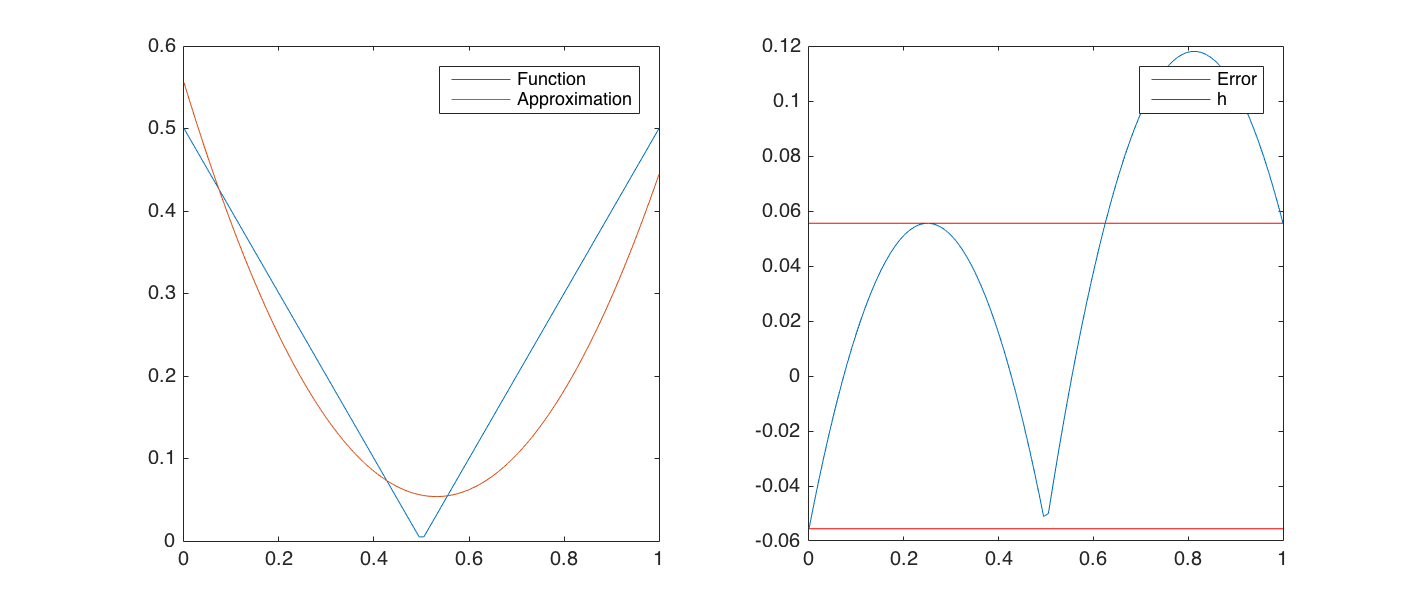
\includegraphics[scale = 0.25]{figtask2hwk4.png}
\caption{Function, approximation and error for the reference \{0, 1/4, 1/2, 1\}}
\label{trialapprox}
\end{figure}
To get a better result, we can take a step of the one point exchange algorithm. We can see that $\eta \approx 0.75$, therefore, following the algorithm (substitute $\eta$ with the $\xi$ that is closest and has the same sign), we have to change the reference to $\{0, 1/4, 1/2, 0.75\}$ obtaining the polynomial $p(x) = 0.5625 -2x+2x^2$ and the plots in Figure \ref{stepexchange}.
\begin{figure}[h]
\centering 
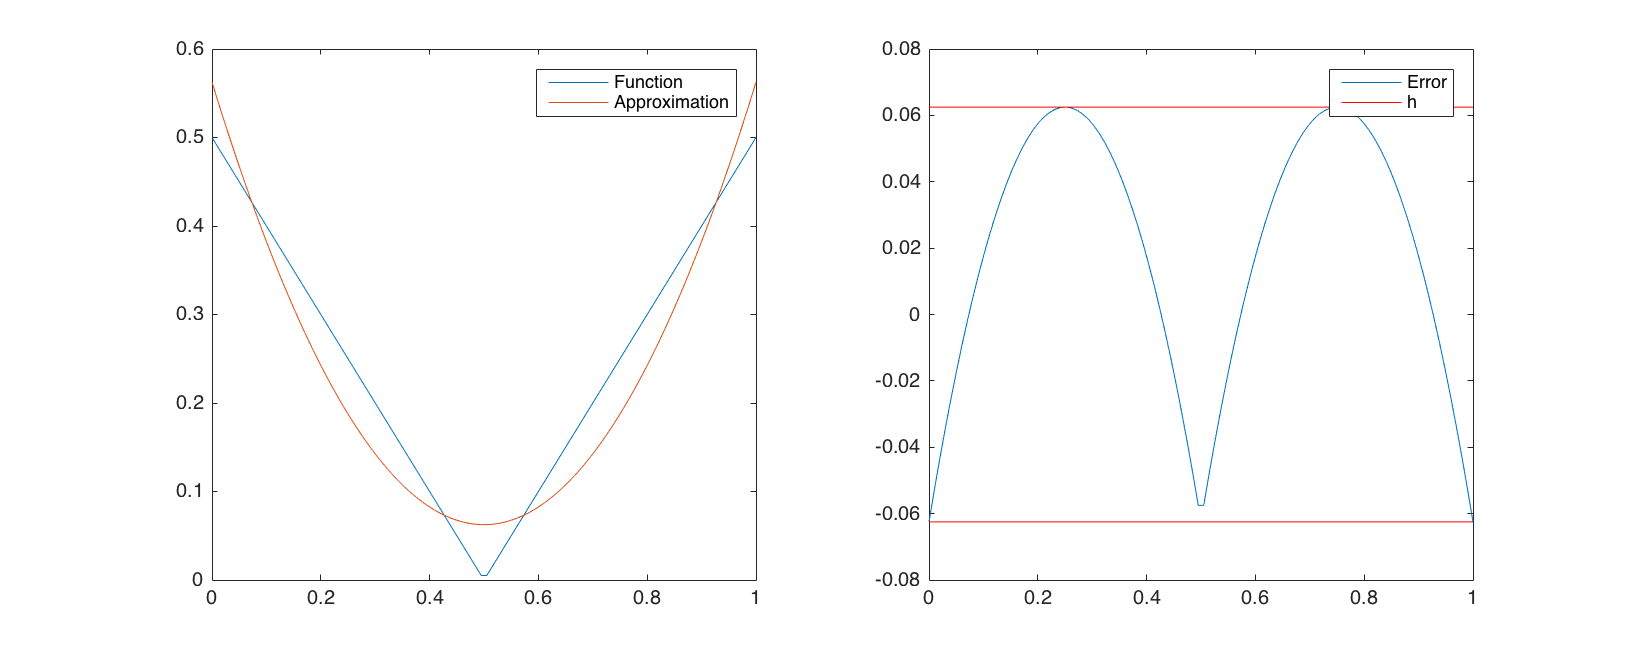
\includegraphics[scale = 0.25]{figtask2hwk4step1.png}
\caption{Function, approximation and error for the reference \{0, 1/4, 1/2, 0.75\}}
\label{stepexchange}
\end{figure}
Now this, if not the best approximation, is very close to what we would want in practice.
\end{solution}

\begin{problem}
  Use a discrete version of the one-point exchange algorithm to
  calculate the best minimax approximation from the space of
  polynomials of degree at most one to the following seven function
  values: $f (0) = 0.3,\, f (1) = 4.2,\, f (2) = 0.1,\, f (3) = 3.4,\, f (4) =
  5.7,\, f (5) = 4.9,\, f (6) = 5.7$. Let the initial reference be the set
  of points $\{0, 3, 6\}$.
\end{problem}

\begin{solution}

\end{solution}

%%% Local Variables:
%%% mode: latex
%%% TeX-master: "report"
%%% End:


\begin{problem}
  Let $\mathcal{A}$ be the 3-dimensional space of functions on
  $[-1,1]$ composed of two straight line segments joined at $x =
  0$. Calculate the element of $\mathcal{A}$ that minimizes
  \begin{equation}
    \label{eq:integral}
\int_{-1}^1 \lvert x^2 - p(x) \rvert \, \text{dx}, \quad p \in \mathcal{A}.
\end{equation}
\end{problem}


\begin{solution}
$\mathcal{A}$ is a Haar space as if a function in $\mathcal{A}$ has
more than 2 zeros it is identically zero. Which can be taken as the
definition of a Haar space.

We then note that equation \ref{eq:integral} is the 1-norm and the
element in $\mathcal{A}$ we are searching for is the best $L_1$
approximation from $\mathcal{A}$ to $x^2$. Now we use our dear theorem
14.5 again, giving us the zeros of the error function. These are given
by equation~\ref{eq:zeros}.
\begin{equation}
  \label{eq:zeros}
\zeta_k = \cos{\left (\pi \left(- \frac{k}{4} + \frac{3}{4}\right)
  \right )}
  \Leftrightarrow
  \begin{cases}
    \zeta_0 = - \frac{\sqrt{2}}{2} \\
    \zeta_1 = 0 \\
    \zeta_2 = \frac{\sqrt{2}}{2} \\
  \end{cases}
\end{equation}

By demanding that the error function have these three zeros we get a
candidate for a best approximation $p^*$ in
equation~\ref{eq:pstar}.

\begin{equation}
  \label{eq:pstar}
  p^*(x)  = 
  \begin{cases}
    - \frac{\sqrt{2} x}{2} & \text{for}\: x \in [-1, 0) \\
    \frac{\sqrt{2} x }{2} & \text{for}\: x \in [0, 1]    
  \end{cases}
\end{equation}

\begin{equation}
  \label{eq:task_4:error}
  x^2 - p^*(x)  = 
  \begin{cases}
    x^{2} + \frac{\sqrt{2} x}{2} & \text{for}\: x \in [-1, 0) \\
    x^{2} - \frac{\sqrt{2} x}{2} & \text{for}\: x \in [0, 1]
  \end{cases}
\end{equation}

The only thing remaining is to check that the criteria, from 14.4, of
there being exactly 3 zeros in the error function is meet. In this
case solving for all the zeros becomes solving a piece wise defined
second order polynomial which is indeed possible. One need not however
solve the equations explicitly. Instead we note that second order
polynomials can have at most 2 zeros and both parts of the error in
equation~\ref{eq:task_4:error} are second order polynomials with one
root in common ($x = 0$). We thus conclude that the error function has
at most 3 zeros and we know by construction that it has 3
zeros. Therefore we know it has {\bf exactly } three zeros. Thus we
have found an element of $\mathcal{A}$ that minimizes
equation~\ref{eq:integral}. Further as $\mathcal{A}$ is a Haar space
the best approximation is unique.

    
% \begin{figure}[!ht]
%   \centering
%   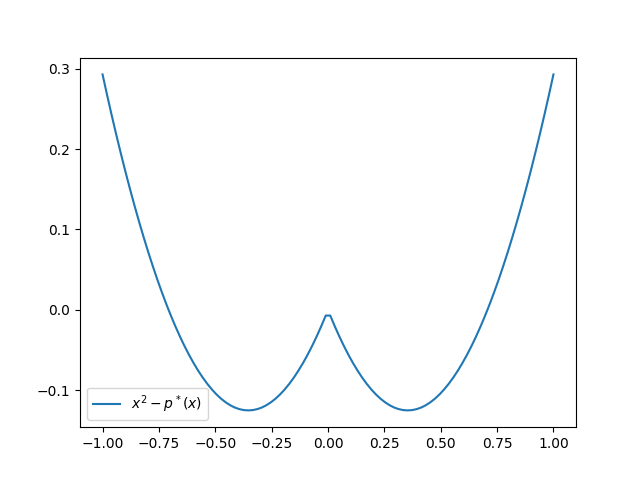
\includegraphics[scale = 0.5]{task_4_error.png}
%   \caption{Plot of $f - p^*$. Note that there is exactly 3 zeros!.}
%   \label{fig:task_3:error}
% \end{figure}

\end{solution}


%%% Local Variables:
%%% mode: latex
%%% TeX-master: "report"
%%% End:


\begin{problem}
Let p be the cubic polynomial that interpolates the function values
$f(0)$, $f(1)$, $f(2)$, and $f(3)$. Express $p(6)$ in terms of $f(0)$,
$f(1)$, $f(2)$, $f(3)$, and verify that your formula is correct when
$f$ is the function ${f (x) = (x − 3) 3 ; 0 ≤ x ≤ 6}$ What is the
uncertainty in the value of $p(6)$, if the uncertainty in each function
value is $\pm \epsilon$?
\end{problem}

%--------------------------------------------------------------------%

\begin{solution}  

\end{solution}

%%% Local Variables:
%%% TeX-master: "report.tex"
%%% End:


\end{document}

%%% Local Variables:
%%% mode: latex
%%% TeX-master: t
%%% End:
